\documentclass[
	% Basic information
	StudentName     = 杨晓宇,
	StudentID       = 1922105012,
	AdvisorName     = 王俊,
	%Grade           = 年级,
	Major           = 信息与计算科学,
	Department      = 理学院,
	% Submit time
	SubmitYear		= 2023,
	SubmitMonth		= 6,
	% Title
	Title           = 加速割平面法的技巧探究,
	TitleEng        = {{Accelerate the exploration of the techniques of the cut plane method}}
]{just_thesis}
%% 以上需要学生把自己的信息填上去的

% 导入页面命令
\newcommand{\inputpage}[1]{
	\input{settings/#1}
}



\begin{document}
	\inputpage{cover}
	
	%%%% 摘要
	\newpage
	\setcounter{page}{1}
	\pagenumbering{Roman}
	\setlength{\headsep}{1.224cm}
	\begin{center}
		\zihao{3}\fakehei 摘\quad 要
	\end{center}
	\vspace{21pt}
	\zihao{-4}
	
	
	\setlength{\baselineskip}{20pt}
% ---------------中文摘要----------------------
	整数规划(Integer Programming , IP)是带整数变量的最优化问题。最大化或最小化全部变量或者部分变量为整数的多元函数受约束于一组等式和不等式条件的最优化问题。整数规划的提出最早可以追溯到上世纪五十年代。近年来,运筹学在日常生活中的应用越来越多,整数规划在工业方面、商业方面、运输方面和经济管理和军事方面都有着重要的应用。我们对于整数规划问题主要的求解方法,目前来说主要是有割平面法和分支定界法。
本文主要阐述了线性规划、整数规划的理论基础,给出了分支定界法与割平面法的具体解题步骤与两种方法的相同点与不同点。之后主要研究如何优化割平面法,并且应用于若干个整数规划实例中,从而达到优化割平面法求解整数规划问题的目的。将整数规划应用于实际生活中解决问题,进一步完善与优化整数规划割平面法。
% ---------------中文摘要----------------------
	\newline
	\newline
	\indent\zihao{-4}{\bfseries 关键词:}\zihao{-4} 线性规划;整数规划;分支定界法;割平面法

%%%%%%%%%%%%%%%%%%%%%%%%%%%%%%%%%%%%%%%%%%%%%%%%%%%% 
	\newpage
	\setlength{\headsep}{1.224cm}
	\begin{center}
		\zihao{3} \textbf{Abstract} 
	\end{center}
	\vspace{21pt}
	\zihao{-4}
% ------------------English Abstract--------------------------
	Integer programming is an optimization problem with integer variables, which maximize or minimize the multiple functions of full or partial variables for integer, subject to a set of equality and inequality constraint optimization problems. The introduction of integer programming can be traced back to the fifties of the last century. In recent years, operations research has been used more and more in daily life, and integer programming has important applications in industry, commerce, transportation, and economic management and military. Our main solution methods for integer programming problems are currently mainly the secant plane method and the branch delimitation method.
This paper mainly expounds the theoretical basis of linear programming and integer programming, and gives the specific problem-solving steps of branching delimitation method and the secant plane method, and the similarities and differences between the two methods. After that, he mainly studied how to optimize the cut plane method, and applied it to several integer programming examples, so as to achieve the purpose of optimizing the cut plane method to solve integer programming problems. Integer programming is applied to solve problems in real life, and the cut plane method of integer programming is further improved and optimized.
% ------------------English Abstract--------------------------
	\newline
	\newline
	\indent\zihao{-4}\textbf{Key Words: }\zihao{-4}\songti Linear programming; integer programming; branch delimitation method; Cut plane method
	
	%%%% 目录
	\newpage
	\setlength{\headsep}{-0.3cm}
	% 去除页码
	\pagenumbering{gobble}
	\tableofcontents
	\clearpage	% 去除页码命令终止
	\setcounter{page}{1}
	\pagenumbering{arabic}

	\setlength{\headsep}{0.624cm}
	\fancypagestyle{plain}{
		\pagestyle{fancy}
	}%在章节页也显示页眉
	\pagestyle{fancy}
	\setlength{\baselineskip}{20pt}
%%%%%%%%%%%%%%%%%%%%%%%%%
	% 第一章绪论
		% **********绪论**************
	{\centering\chapter{绪论}}
	\setlength{\baselineskip}{20pt}
%%%%%%%%%%%%%%%%%%%%%%%%%%%%%%%%%%%%%%%%%%%%%%%%%%%%

	
	\section{课题背景}
	
线性规划\cite{yangchang2014integer}(Linear Prigramming 简记为LP)是运筹学数学规划中研究较早、发展较快、应用广泛的一个非常重要的分支。线性规划,顾名思义,是由两个关键部分构成,也就是线性与规划,线性是如果一个函数  满足下面可加性与齐次性这两个条件,那么则说明该函数是线性的。
  
  
我们也经常地把一阶多项式函数  称为线性地,其中 是常数。
线性规划自从1947年由G. B. Dantzig提出了解决线性规划问题的单纯形法之后,线性规划问题理论不断趋于成熟,在实际应用当中,由于计算机能够处理多个约束条件和决策变量的线性规划问题,线性规划成为现代管理经常运用的方法之一,我们在解决实际问题时,要把问题转化成为一个线性规划数学模型,我们需要选取恰当的决策变量建立模型,一般来说,线性规划问题的标准型为:
	\begin{equation*}
		\begin{split}
			&\max_{x \in \mathbf{R}^{n}}~z = \sum_{j=1}^{n}c_j x_j \\
			& \quad \text{s.t.} ~
				\begin{cases}
					\sum_{i=1}^{n} a_{ij} x_j = b_i, ~&i = 1, 2, \cdots, m; \\
					x_j \geq 0, ~&j = 1, 2, \cdots, n.
				\end{cases}
		\end{split}
	\end{equation*}

线性规划如今在现实生活中的应用极多,比如,在生产方面,为了适应社会不确定的需求计划,需要利用线性规划的理论方法和仿真模拟方法来估算确认产方的生产值和劳动力分配;在车辆调度问题方面,也可以运用线性规划对城市车辆进行调研分析,对于交通堵塞的情况做出优化路线。

	
	\subsection{线性规划问题的概念}
	
	说到整数规划\cite{ywy2022},就会想到线性规划,线性规划表示所有的约束条件与目标函数皆线性,未知数的次数都是一次,线性规划中包含着线性整数规划。线性规划求解问题的基本方法有单纯形法、改进单纯形法、对偶单纯形法等。而整数(线性)规划是线性规划中未知数只能取整数的特例,它在线性规划的基础上增加了整数约束。整数线性规划可以分为以下类别:
	
	(1)纯整数线性规划,
	
	(2)混合整数线性规划,
	
	(3)0-1型整数线性规划;
	
	其中纯整数线性规划是指全部的决策变量都要取整数值的整数线性规划;混合整数线性规划是指决策变量当中有部分取整数值,另一部分可不取整数值的整数线性规划;0-1型整数线性规划是只决策变量取值0或者1的整数线性规划。
	
线性规划实际就是求解连续变量的线性优化问题,相比线性规划,整数规划是求解整数变量的优化问题,我们研究较多的问题是纯整数线性规划和混合整数线性规划(MILP),与线性规划不同的是,整数规划它所强调的是它的决策变量取值需要为整数,而求解线性规划的方法有时不能保证求得的解满足整数规划的整数条件,所以求解整数线性规划需要使用它的对应方法,我们较为常见的就是分支定界法和割平面法。

	
	\subsection{整数规划问题的概念及分类}
	
	分支定界法(Branch and bound),该方法是20世纪60年代由理查德.卡普(Richard Karp)所提出,理查德.卡普还研究过最大网络流问题,发表了“组合问题中的可归约性”(Reducibility among Combinatorial Problems)重要论文。 分支定界法较为灵活,便于使用计算机求解整数规划。方法命名上就知道此方法核心点就是分支和定界,其中分支是将一个问题细分成为若干个子问题,然后逐个的讨论这些子问题;定界是指在分支过多的情况下,我们需要讨论的情况也变得越来越多,这时便需要定界,在满足(1)得到最优解,(2)根据现有的条件能够排除最优解在这个分支当中,二者其一,就可以定界,达到删除无讨论意义的分支,从而讨论有意义分支的目的。
使用分支定界法来求解整数规划的步骤如下:

(1)	求解整数的松弛问题的最优解

若该最优解为整数,则直接得到整数规划最优解
若该最优解不为整数,则进行下个步骤

(2)	分支定界
我们从不满足整数条件的基变量当中任选一个Xi来进行分支,这个分支必须满足xl ≤[xl ] 或xl ≥[xl ] +1中的任意一个,我们把这两个约束条件加入原问题,从而形成了两个互不相容的子问题(即二分法)。

“分支”为求解整数规划最优解创造条件,“定界”可以来提高搜索的效率。

	
	\subsection{分支定界法概念及运用方法}
	
	割平面法(cutting plane method)是1958年由美国的高莫利(R.E.Gomory)所提出,故而又称为Gormory割平面法,是计算整数规划的另一种常用方法,此方法相较于分支定界法,它的计算量要小很多,不需要每次计算都分两种情况来进行讨论,但他们的相同点都是把整数规划问题转化成为线性规划问题来解决。割平面法的基本思路如下:首先并不去考虑整数性约束条件,直接求解对性的线性规划问题,如果求解线性规划问题得到的最优解恰好是整数,则结束计算,此解为整数规划问题的最优解,如果不是整数,则增加割平面,要满足两个条件:(1)从线性规划问题的可行域当中至少割掉非整数最优解;(2)不能割掉任何整数可行域;之后再缩小的可行域当中继续求解线性规划问题,经过有限次切割,在不断缩小的可行域中的一个整数极点上达到整数规划求解的最优解。
使用割平面法来求解整数规划的步骤如下:

(1)	首先不考虑变量的取整约束,将原问题的数学模型进行标准化,使用单纯形法求解线性规划问题,假使求得最优解非整数则转至下一步。

(2)	将一个“切割不等式”添加到整数规划的约束挑花那种,对上述线性规划问题的可行域进行“切割”。

割平面法的关键就是我们要如何找当适当的割平面方程,我们此课题主要研究就是如何优化割平面法求解整数规划问题。

	
 
	\section{国内外研究现状}
	
	运筹学如今在农业、工业、经济和社会问题等领域都有广泛的应用,而运筹学体系也不断地发展,形成运筹学多个分支,比如有数学规划(线性规划、非线性规划、整数规划、目标规划、动态规划、随即规划等)、图论与网络、排队论、存贮论、对策论、决策论、维修更新理论、搜索论、可靠论和质量管理等方面。
线性规划最早是由法国数学家J.-B,-J,傅里叶于1832年提出的想法,之后C.Valle Pogson在1911年也提出了线性规划的数学想法,但都没有引起人们的注意。直到五十年代之后,出现了一大批研究线性规划问题的理论。在1954年C.Lamkey提出了对偶单纯形法,这是对于解决线性规划问题的一个重要方法,同年,S.加斯等人解决了对于线性规划问题中对于参数规划和灵敏度问题的的分析问题,在1956年,A.塔克提出了互补松弛定理由,G.B.Danzik与P.沃尔夫为分解算法提供了理论知识,八十年代印度数学家N.卡玛卡提出了新的多项式时间算法,这对于求解线性规划问题非常有效。

割平面法是由高莫瑞(R.E.Gomory)1958年提出的,故又称Gomory割平面法,经过三十多年的发展,已经不断出现了很多解决整数规划问题的方法。如今人们大多使用分支定界法和割平面法求解整数规划,割平面法相较于分支定界法,计算量要小许多,不用每次都要分两种情况进行讨论,而是用它特有的简便方法进行选择。

目前多数运筹教科书关于割平面的讲解不够深入,关于加快割平面法的速率只有提出在实际解题时,经验得出若从最优单纯形表中选择具有最大小(分)数部分的非整分量所在行构造割平面约束,往往可以提高“切割”效果,减少“切割”次数。

国内对于运筹学的研究始于上个世纪八十年代,钱颂迪、胡运权结合运筹学,运用线性规划、数学模拟方法来解决生产应用中的合理下料、配料问题,并且应用在物料管理方面。李军、张锦运用了线性规划来解决物流运输当中汽车路线择优的问题。郭耀煌、陈唐民结合了线性规划理论和多目标决策理论,重点解决了车辆调配或者物流运输当中最短时间的数学问题。左永林、柳志新运用动态规划理论解决了供料方案的优化研究的问题。

经过半个世纪我国数学快速发展,但还是习惯性使用给定方法计算数学问题,在使用割平面法求解整数规划问题时,只是运用选取最大分数部分的非整分量所在行构造割平面约束,但如果遇到存在多个最大分数部分相同的情况,大多数是任选一个非整分量所在行来构造割平面约束,导致切割次数增加,无法快速找到最优解。

	
	\section{本文主要研究内容}
	
	1、收集和分析相关信息,翻译好论文文献并翻阅关于整数规划割平面法的论文,将与我们研究课题相关的部分划上重点,对于优化割平面法的部分进行着重分析,针对整数规划问题的研究有利于加强我们对割平面法求解整数规划的认识,可以完善有关割平面法使用的研究。
	
2、利用单纯形法求解松弛问题,观察所给课题题目的松弛问题的最优解是否满足整数条件,假使不满足整数条件,则要继续求解该问题,分别使用分支定界法与割平面法进行该课题例题的解答,并列出相应步骤,对比分析两种方法的相同点与不同点。

3、利用书中所提出的方法选取具有最大小(分)数部分的非整分量所在行构造Gomory约束,由于所给题目具有特殊性无法选择最大非整分量,将两个最大小数非整分量所在行都提取出来构造割平面约束,对比两个约束的结果,根据结果同整数之间的差,选择切割条件较强的Gomory约束,观察规律,给出假设。

4、证明所给假设的正确性。


	\section{本文研究方法}

1、文献研究法:本课题的研究需要阅读查阅大量的文献成果,才能总结出现在该论题的研究情况,我们要寻找出以前研究的不足处和避免论文研究内容的重复性。通过上网查阅或者是图书馆借阅有关于研究整数规划割平面法的书籍文献或论文资料,并且对于重要的内容进行提要分析,从而了解掌握所要研究的割平面法的研究现状,进一步全面地、正确地了解掌握割平面法。

2、实例证明法:在论文中,对于各种求解整数规划问题的方法进行对比分析,结合实际对割平面法进行分析,结合运筹学理论分析如今割平面法求解问题de 发展现状,以及割平面法的特征及优劣点,依据已有的科学理论,以及应用割平面法求解相应课题的实例,提出关于优化割平面法的假想,并且将该猜想作用于各种典型题目,对加快割平面法探究的假想进行证明。

 


	\section{本文研究步骤}
	
	1、利用分支定界法求解给定题目的整数规划问题,使用图解法求出松弛问题的最优解,之后进行分支定界求解最优整数解;割平面法求解给定题目的整数规划问题,使用单纯形法求解松弛问题,增加割平面约束,给出每个步骤的单纯形表,比较两种方法的优劣点,着重分析割平面法求解步骤。
	
2、进行文献检索、阅读与总结,了解割平面法相关内容,知晓相关领域有影响的成果及其内容,并且要避免研究的重复性,总结以往论文的不足之处,并且想办法优化,在此基础上提出优化割平面法的合理假设,并将其应用于各类典型整数规划例题中,以此证明该假设是否成立。

3、确定研究的方法,参考多个经典例题,推导出加快割平面法探究的猜想,并落实研究,进行可行性分析,对于该猜想进行证明。

4、得出结论,完成论文。

	
	% 第二章主要结论
		{\centering\chapter{加速割平面法的技巧探究}}

\section{具体求解整数规划例题}
求解如下的整数线性规划:
	\begin{equation}\label{Chapter2ExamILP}
		\begin{split}
			&\max_{x \in \mathbf{R}^{2}}~z = 2 x_1  + 3 x_2  \\
			& \quad \text{s.t.} ~
				\begin{cases}
					3x_1 + 5x_2 &\leq 15; \\
					3x_1 + x_2 &\leq 6;\\
					x_1, x_2 \geq 0, &x_1, x_2 \text{为整数} 
				\end{cases}
		\end{split}
	\end{equation}

求解的过程中发现,增添的“割平面”不能有效地提高得到最优解的速度,而且目标函数值也下降的非常缓慢。
针对以上描述的具体问题,要求同学们按照已有的知识积累,请提出一个解决上述问题的改进方法,找出或者时尝试性地给出相应的改进技巧,来加速“割平面法”的求解速度。

\subsection{分支定界法求解整数规划}

求解如下的整数线性规划:
	\begin{equation*} 
		\begin{split}
			&\max_{x \in \mathbf{R}^{2}}~z = 2 x_1  + 3 x_2  \\
			& \quad \text{s.t.} ~
				\begin{cases}
					3x_1 + 5x_2 &\leq 15; \\
					3x_1 + x_2 &\leq 6;\\
					x_1, x_2 \geq 0, &x_1, x_2 \text{为整数} 
				\end{cases}
		\end{split}
	\end{equation*}

求解的过程中发现,增添的“割平面”不能有效地提高得到最优解的速度,而且目标函数值也下降的非常缓慢。
针对以上描述的具体问题,要求同学们按照已有的知识积累,请提出一个解决上述问题的改进方法,找出或者时尝试性地给出相应的改进技巧,来加速“割平面法”的求解速度。

\subsection{割平面法求解整数规划}

第一步,使用单纯形法求解松弛问题
检测LP的初始单纯形表1.1
表1.1  LP的初始单纯形表
 
 虽然初始单纯形法表的检验数都是非负的,但是结果不是期望的,按照字典顺序法选择入基变量 ,计算 ,因此选择出基变量 
 

在最后的单纯形表
 
把上述左边的变量系数都分解为带有真分数形式,即
 
第二步,寻找Gomory约束,应该选取切割条件较强的约束
若选取 ,则对应这一行的约束为
 
对应的Gomory约束为          
 
若选取 ,则对应这一行的约束为
 
对应的Gomory约束为


\section{探讨分支定界法求解整数规划}

根据上述例题综,我们从分支定界法和割平面法两种方法的实质和例题解题步骤、适用对象等方面做了介绍,从中我们发现运用分支定界法是非常灵活且便于计算机求解的,但是同样,我们也发现,分支定界法的缺点是必须在每一个节点解一个完整的线性规划问题,假使我们的题目是一个大型问题,那么使用分支定界法求解那将是一个十分耗时的工程,且并不是每一个整数规划都能用分支定界法来求解。下面来看一个例子:
  
首先我们先求该整数规划问题的松弛问题,即
 
根据单纯形法求得该松弛问题的最优解为  ,此时的最大值  ,也就是它的初始上界为  ,但是很明显,所得到的最优解并不满足整数条件,因此我们应该继续确定 的的下界 ,假使容易求得一个整数解,那么就可以把这个值作为初始的下界,反之则可以令初始下界为  或者式等到使用分支定界法给出一个整数可行解之后再给出,它的作用就是解的目的仅在于求得比该下界更好的目标值,在此例子中,我们有  .

接下来我们就需要运用分支定界法来求解该问题,首先我们分出各支并求解相应各支的解,我们可以使用图解法便于观看,我们先选取较小的解,即取 ,根据分支定界法使用条件,我们要在原问题上增加两个约束,即要分别增添  形成两个分支,然后我们再分别求解这两个分支的解,当然在求解的过程中我们可能会遇到一些情况:

假使该分支没有可行解,则我们不再对其分支;假使在该分支的最优解得到了整数解,则该分支停止;假使该分支得到非整数解,则要继续分析,如果得到的 值比初始下界还要小,则我们没有必要再对其分支,反之继续分支。当我们遇到这一对分支都需要继续向下分解的情况,那么假如我们求解的目标值是求其极大值,那么我们先将分支中目标函数较小的那一分支暂时搁置,然后分解另一目标函数值较大的分支,直到求解完毕,然后再将留待处理的分支按照“后进先出”的原则对其依次分解求值。

需要注意的是在每次分支求解时,修改原来的上、下界,我们可以每当求出一个新的整数解,就将其对应的目标函数值与之前的进行对比,取最大的,而下界也应在不断的求解中增大(在求目标值为极大值的情况下)。

该例题的分支过程图如下:

\section{加速割平面法的技巧探究}

平面法不断地增加线性约束条件(几何术语称为割平面),从而将原规划问题地可行域割掉一部分,使得切割掉的部分只包含有非整数解,而并没有切割任何整数可行解,就这样不断切割知道得到地可行域有一个整数坐标地极点,它恰好是所求问题的最优解,割平面法对于求解整数规划问题是很有效的,但是从前面的计算过程我们可以发现,同一张单纯形表可以产生不同的切割不等式,那么哪一个不等式的切割效果更好呢?这是一个值得探讨的问题。

我们无法根据某些例题来武断的评判分支定界法与割平面法谁优谁劣,两种方法各有千秋,他们的共同点都是对于可行域切割,刨除掉一部分非整数解域,使得剩下的子域中包含原来整数规划问题的所有可行域,而他们的不同点就在于,割平面法切割剩下的子域仍为一个,而分支定界则是两枝。割平面法对于问题的结构以及求解结果有着较高的要求,也就是要区分纯整数和混合整数问题,不同问题有不同的切割方程,在切割后剩下的仍然是一个子域,后续的计算是一个较小的子域上的整数规划问题,而分支定界法在作分割之后分成了两个分支,后续的计算就是小哥比较小的子域上面的整数规划问题,但是随着分支增多,计算量也越来越大,我们计算时要具体问题具体分析,而下面我们来着重研究一下割平面法。


\subsection{研究常用割平面法优化技巧}

在我们之前的运筹学学习中,我们已经知道了一种优化割平面法选取约束方程的方法,即选取单纯性表中具有最大小(分)数部分的非整分量所在行来构造Gomory约束,那么为什么会有这个方法呢?下面我们来看:
在我们使用割平面法求解整数规划问题时:


使用割平面法来求解上述整数规划问题,首先就需要来求解其松弛问题的最优解,也就是说,我们先不去考虑上述问题中的整数约束条件,直接使用单纯形法求解线性规划问题,得到问题的最优解,假使我们得到了整数最优解,则问题得到解决,所求得的最优解就是原整数规划问题的最优解;然而我们在计算中,松弛问题的最优解往往不能满足其整数约束条件,那么我们就需要增加割平面,几何上来说就是将线性规划可行域切割掉一部分,被切割下去的部分不包括任何整数可行解。之后就是在缩小的可行域上继续求解线性规划问题最优解,我们通过不断地增加割平面方程,使得可行域不断缩小,直到找到原整数规划问题的最优解,那么我们研究的重点也就是如何寻找适当的割平面方程。
下面我们来考虑纯整数规划问题 


\subsection{割平面法改进方案}

在使用割平面法求解纯整数规划问题的时候,我们使用传统的选取割平面方法,即选取非整分量分数部分最大的基变量所在行,但是我们也会遇到一些特殊的情况,比如得到的单纯形表中存在不只一个最大非整分量分数,那么这个情况下,一般来说我们会任意选取一个来做,但是并不清楚哪个割平面方程的约束性更强,就比如我们课题给出的题目,常常切割次数很多,运算量太大,难以快速的找到整数规划最优解。而我们从表3中可以看到割平面选取与 有关,那么将多个最大非整分量分数所在行提取出来列成割平面方程,方程右式分数部分相同,那么我们就可以观察方程左式,我们不妨假设选取最大左式中的系数相加提取其分数部分所在割平面方程,也就是在右式相同的情况下来比较左式系数相加的绝对值中的分数部分,值越大,其所在割平面方程的切割条件越强,下面是运用该改进方法求解整数规划的算法流程图:





	% 第二章主要结论
		{\centering\chapter{数值实验}}
	
	本科生毕业设计(论文)的正文是主体部分,要着重反映自己的工作,突出新的见解,例如新思想、新观点、新规律、新研究方法、新结果等。正文可以包括:调查对象、实验和观测方法、仪器设备、材料原料、实验和观测结果、计算方法和编程原理、数据资料、经过加工整理的图表、形成的论点和导出的结论等。
	
	正文要求论点正确,推理严数据可靠,文字精练,条理分明,文字图表清晰整齐。利用别人研究成果必须附加说明。引用前人材料必须引证原著文字。在论文的行文上,要注意语句通顺,达到科技论文所必须具备的"正确、准确、明确"的要求。
	
	由于研究工作涉及的学科、选题、研究方法、工作进程、结果表达方式等有很大的差异,不对正文内容作统一硬性的规定。但是,必须实事求是,合乎逻辑,层次分明。

\begin{lemma}\label{LemmaLbeta}
	Let $\left\{ \mathbf{x}^{k}, \mathbf{y}^{k}, \mathbf{z}^{k} \right\}$ be the sequences denoted by {\tt ADMM}$_{\ell_{1}/\ell_{\infty}}$, and then we have 
	\begin{equation} 
			\mathcal{L}_{\beta} \left( \mathbf{x}^{k+1}, \mathbf{y}^{k+1}, \mathbf{z}^{k+1} \right) \leq  \left(\frac{\lambda_{\min}  \left( \mathbf{A}^{\top} \mathbf{A} \right)}{2}  +  \frac{\beta}{2} - \frac{L_f^2}{\beta} \right) \left \Vert \mathbf{y}^{k+1} - \mathbf{y}^{k} \right \Vert_{2}^{2},
	\end{equation} 
	where $L_f \triangleq \lambda_{\max} \left( \mathbf{A}^{\top} \mathbf{A} \right)$ and  $\lambda_{\min}  \left( \mathbf{A}^{\top} \mathbf{A} \right) > 0$  is the largest and non-negative smallest eigenvalue of $ \mathbf{A}^{\top} \mathbf{A}$, respectively.
\end{lemma}
	
	\section{格式要求}
	 
\begin{proposition}\label{LemmaLbeta1}
	Let $\left\{ \mathbf{x}^{k}, \mathbf{y}^{k}, \mathbf{z}^{k} \right\}$ be the sequences denoted by {\tt ADMM}$_{\ell_{1}/\ell_{\infty}}$, and then we have 
	\begin{equation} 
			\mathcal{L}_{\beta} \left( \mathbf{x}^{k+1}, \mathbf{y}^{k+1}, \mathbf{z}^{k+1} \right) \leq  \left(\frac{\lambda_{\min}  \left( \mathbf{A}^{\top} \mathbf{A} \right)}{2}  +  \frac{\beta}{2} - \frac{L_f^2}{\beta} \right) \left \Vert \mathbf{y}^{k+1} - \mathbf{y}^{k} \right \Vert_{2}^{2},
	\end{equation} 
	where $L_f \triangleq \lambda_{\max} \left( \mathbf{A}^{\top} \mathbf{A} \right)$ and  $\lambda_{\min}  \left( \mathbf{A}^{\top} \mathbf{A} \right) > 0$  is the largest and non-negative smallest eigenvalue of $ \mathbf{A}^{\top} \mathbf{A}$, respectively.
\end{proposition}

	\section{图、表格和公式要求}
	
	文中的图、表、附注、公式一律采用阿拉伯数字分章编号。如:图2-5,表3-2,等。
	
	\subsection{图格式要求}
	
	插图须精心制作,线条清晰、美观,不得徒手画图,必须按国家规定标准或工程要求用计算机绘制。插图应与正文呼应,切忌与文字表述重复。不得插入与正文无关的图表或照片。插图应有图题,图序及图名居中置于图的正下方,图中的术语、符号、单位等应同文字表述一致。插图为嵌入型居中排列。图中字体及大小根据实际情况自行调整。
	
	\begin{figure}[h]
%		\bicaption{中文图名}{英文图名}\label{tab:fig1} % 放在这里,标注在表上面
		\centering
		\subfloat[\zihao{5}图a标题]{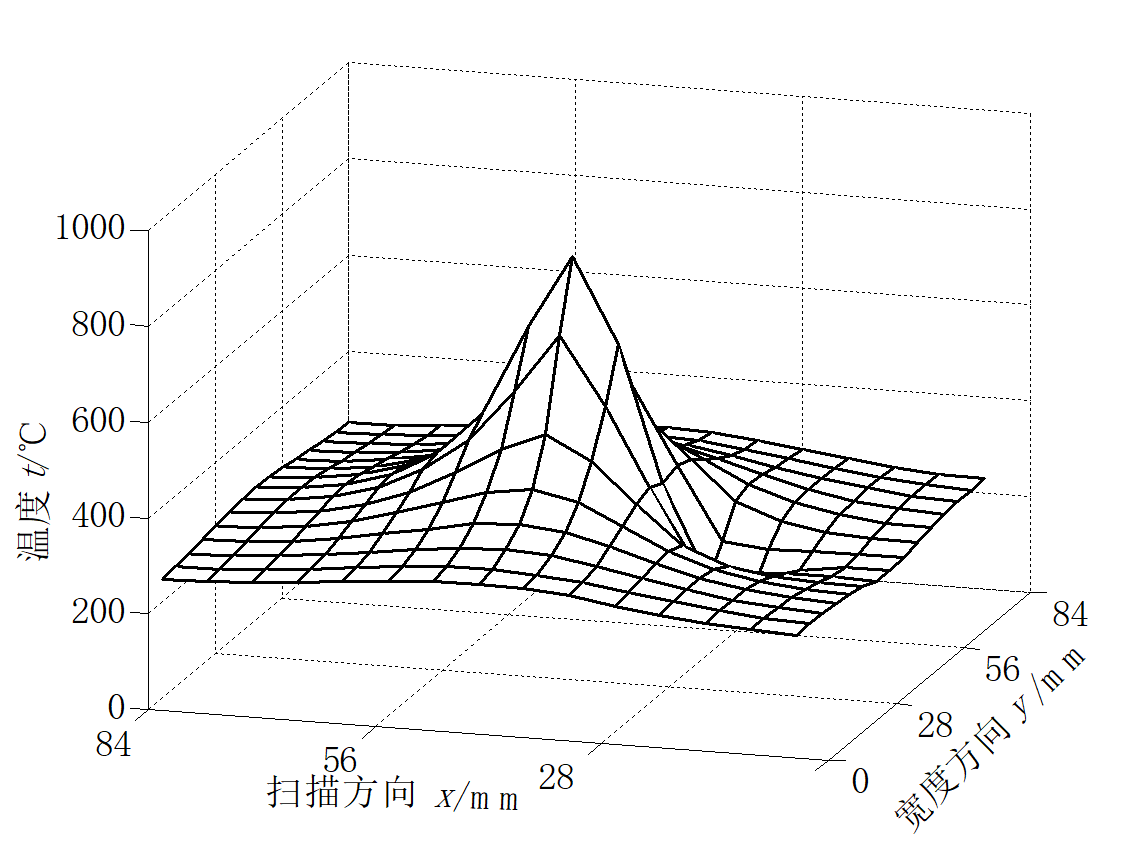
\includegraphics[width=0.4\textwidth]{fig21a.png}\label{fig1}}\hspace{30pt}
		\subfloat[图b标题]{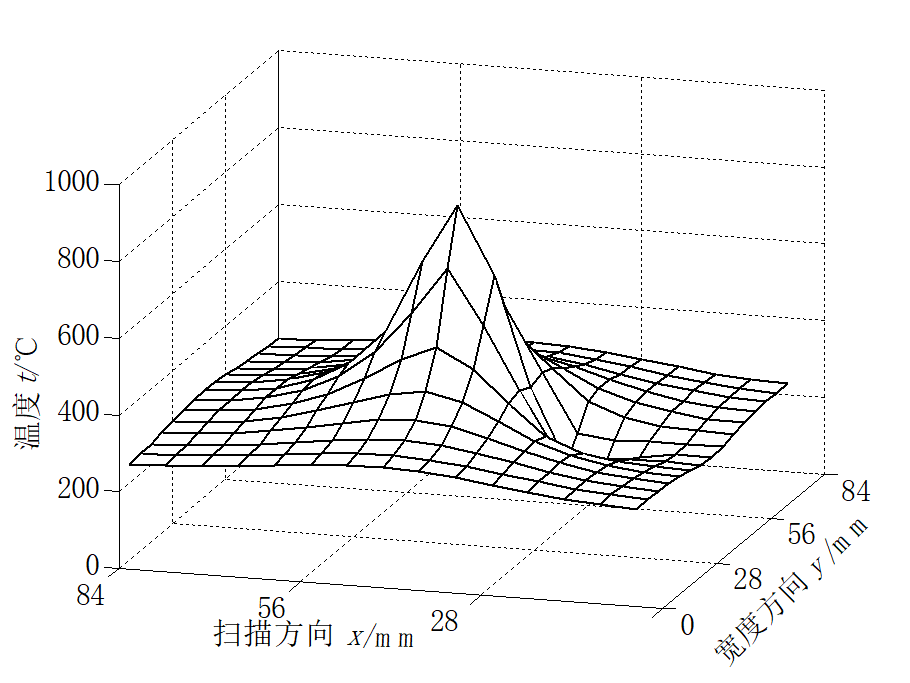
\includegraphics[width=0.4\textwidth]{fig21b.png}}
		\bicaption{中文图名}{英文图名}\label{tab:fig1} % 放在这里,标注在表下面
	\end{figure}
	
	\subsection{表格式要求}
	
	表中参数应标明量和单位的符号。表中字体及大小根据实际情况自行调整。行间距为单倍行距。表序号及表名称置于表的上方。
	
	表名称:正文中的表要有中文名称,表的中文名称为5号宋体字,不加粗,居中并位于表上;
	
	表尺寸:表尽量以一页的页面为限,一旦超限要加续表;
	
	表位置:表居中排列;
	
	表格式:三线表。三线表的组成要素包括:表序、表题、项目栏、表体、表注。三线表通常只有3条线,即顶线、底线和栏目线。其中顶线和底线为粗线,栏目线为细线。如下表:
	
	\begin{table}[!ht]
%		\bicaption{中文图名}{英文图名}\label{tab:lable} % 放在这里,标注在表上面
		\begin{tabular*}{\hsize}{@{}@{\extracolsep{\fill}}lllllllllllll@{}}
			\toprule
			$p_{t}$  &21  &22  &20  &15  &10  &8   &5   &10  &18  &10  &14  &18\\
			\midrule
			$c_{t}$  &5   &13  &10  &10  &10  &10  &10  &10  &10  &10  &10  &10\\
			$h_{t}$  &10  &5   &5   &5   &5   &5   &5   &5   &5   &5   &5   &5 \\
			$s_{t}$  &100 &100 &100 &100 &100 &100 &100 &100 &100 &100 &100 &100\\
			$d_{t}$  &30  &45  &50  &55  &45  &55  &90  &80  &90  &65  &80  &70 \\
			\bottomrule
		\end{tabular*}
		\bicaption{中文图名}{英文图名}\label{tab:lable} % 放在这里,标注在表下面
	\end{table}
	
	\subsection{公式}
	 
	
	% 第二章主要结论
		{\centering\chapter{结论}}
	
	由研究课题题目假设,最终单纯形表中基变量,也就是b,改为整数与真分数相加的形式,比较大小,更大的其收敛条件更强,这是书本上的话,但课题第一次单纯形法计算出的b的真分数部分相等,于是再次假设如果具有两个或两个以上的真分数相等,则将单纯形表表示为Gomory收敛条件的形式,右式真分数不变,此时各式中它们是相等的,分别将左式中的系数相加,所得的数字取绝对值,转换成整数与真分数相加的形式,将各式真分数进行比较,大的其收敛条件更强。为探究此假设成立的非偶然性,随机选取了上面例题,我们的假设仍旧成立,由此达成优化割平面法解决整数规划问题的目的。所以在使用割平面法求解整数规划问题的时候,我们就可以使用此优化方法来减轻计算负担。
	
综上所述,本论文主要探讨了对于割平面的优化改进方法,首先就是我们经常用的,在使用割平面求解整数规划问题时,选取非整数解变量中分数部分最大的一个基变量,然后取其相应行来构造割平面,然后放入原来的线性规划问题中,继续使用单纯形法求解最优解问题,我们也证明了其正确性,并且给出了影响最优解的因素。而我们在求解过程中,也会遇到一些特殊情况,比如当非整数解变量中分数部分最大的基变量有两个或者两个以上的时候,我们就要对于这几行的非基变量分别相加,取它们的真分数部分,并进行比较,从中选取最大真分数行来作为割平面,它是切割条件较强的Gomory约束,从而来减少割平面的切割次数和运算计算量,更快的找到最优解。


%%%%%%%%%%%%%%%%%%%%%%%%%%%%%%%%%%%
 \begin{algorithm}[th!]
\SetAlgoLined
	\caption{Alternating Direction Method of Multipliers  for the $\ell_{1}/\ell_{\infty}$ minimization   ({\tt ADMM}$_{\ell_{1}/\ell_{\infty}}$)}
	\label{ADMML1inf}
	\KwIn{ The initial points: $\mathbf{y}^{0} =\mathbf{z}^{0} \in \mathbb{R}^{n}$, the relative error $\varepsilon = 10^{-8}$, {\tt IterMax} $=100n$, $\lambda = 10^{-4} $ and $\beta  =L_0 =  2\lambda_{\max} \left( \mathbf{A}^{\top} \mathbf{A} \right) $.}
 
	\While{ $k < ${\tt  IterMax}  or $ \frac{\Vert \mathbf{x}^{k} - \mathbf{x}^{k-1} \Vert_2}{ \Vert \mathbf{x}^{k} \Vert_2} >\varepsilon$}{
 		\begin{itemize}
 		\item[(1)] Compute 
			\[
			 \mathbf{v}^{k} = \mathbf{y}^{k} -  \frac{\mathbf{z}^{k}}{\beta},
			 \]
		if $\beta  < \lambda \max \left\{ 	\frac{\Vert \mathbf{v}^{k} \Vert_{0} - \vert \mathcal{I}_{\max}\left( \mathbf{v}^{k} \right) \vert}{ \Vert \mathbf{v}^{k} \Vert_{1}\Vert \mathbf{v}^{k} \Vert_{\infty} } , \frac{1}{\Vert \mathbf{v}^{k} \Vert_{\infty}^{2} } \right\}$ then
		\[
					\beta  = L_0  + \lambda  \max \left\{ 	\frac{\Vert \mathbf{v}^{k} \Vert_{0} - \vert \mathcal{I}_{\max}\left( \mathbf{v}^{k} \right) \vert}{ \Vert \mathbf{v}^{k} \Vert_{1}\Vert \mathbf{v}^{k} \Vert_{\infty} } , \frac{1}{\Vert \mathbf{v}^{k} \Vert_{\infty}^{2} } \right\},
		\]
		else $\beta  = L_0$ end.
	\item[(2)] Calculate $\mathbf{x}^{ k+1}, \mathbf{y}^{ k+1}$ and the dual variable $\mathbf{z}^{ k+1}$ via
			\[
			\begin{cases}
		 \mathbf{x}^{ k+1} &= \sign\left( \mathbf{v}^{k} \right) \odot \max \left\{  \left\vert \mathbf{v}^{k} \right\vert -\frac{\lambda}{\beta \Vert \mathbf{v}^{k} \Vert_{\infty} } , 0\right\} ,\\
		 \mathbf{y}^{ k+1} &=  \left(  \mathbf{ I}_{n}  - \frac{1}{\beta } \mathbf{A}^{\top}  \left( \mathbf{I}_m  + \frac{1}{\beta } \mathbf{A}\mathbf{A}^{\top}\right)^{-1}  \mathbf{A}\right)  \left( \frac{\mathbf{A}^{\top} \mathbf{b}}{\beta } + \frac{\mathbf{z}^{k}}{\beta } + \mathbf{x}^{k+1} \right),\\
		\mathbf{z}^{ k+1} &=  \mathbf{z}^{ k} + \beta \left( \mathbf{x}^{ k+1} - \mathbf{y}^{ k+1} \right)  .
	 \end{cases}
	  \]  
	  and update again
	  \[
	  		 \mathbf{x}^{ k+1}_{i} = \mathbf{v}^{k}_{i},~i \in   \mathcal{I}_{\max}\left( \mathbf{v}^{k} \right)
	  \]
		\item[(3)] Update $k = k +1.$
	  \end{itemize}
	}
 \KwOut{ Finally solution $\mathbf{x}^{ k+1}$.}
\end{algorithm}
	
%%%%%%%%%%%%%%%%%%%%%%%%%%%%%%%%%%%%%%%%%%%%%%%%%%%%

	% -----------使用bib文件储存参考文献信息------------
 % {\centering \bibliography{just_refs.bib}}
%	\addcontentsline{toc}{chapter}{参考文献}%将“参考文献加入目录中”
%	\bibliographystyle{gbt7714-2005-numerical}

%% 参考文献也可以采用另外一种方式:
{\centering 
\addcontentsline{toc}{chapter}{参考文献}%将“参考文献加入目录中”
\begin{thebibliography}{2}
\providecommand{\natexlab}[1]{#1}
\providecommand{\url}[1]{#1}
\expandafter\ifx\csname urlstyle\endcsname\relax\else
  \urlstyle{same}\fi
\expandafter\ifx\csname href\endcsname\relax
  \DeclareUrlCommand\doi{\urlstyle{rm}}
  \def\eprint#1#2{#2}
\else
  \def\doi#1{\href{https://doi.org/#1}{\nolinkurl{#1}}}
  \let\eprint\href
\fi

\bibitem{yangchang2014integer}
杨明歌,常水珍.
\newblock 求解整数规划的割平面法的研究\allowbreak[J].
\newblock 洛阳师范学院学报, 2014, 33\allowbreak (05): 201-213.
\newblock DOI:  \url{10.16594/j.cnki.41-1302/g4.2014.05.001}.

\bibitem{ywy2022}
殷允强,王杜鹃,余玉刚 主编.
\newblock 整数规划:基础、扩展及应用\allowbreak[M].
\newblock 北京: 科学出版社, 2022.

\bibitem{bian2012smooth}
Wei Bian, Xiaojun Chen.
\newblock Smoothing Neural Network for Constrained Non-Lipschitz Optimization With Applications\allowbreak[J].
\newblock IEEE Transaction on Neural Networks and Learning Systems, 2012, 23\allowbreak (04): 399-411.
\newblock DOI:  \url{ 10.1109/TNNLS.2011.2181867}.


\end{thebibliography}}
 
%%%%%%%%%%%%%%%%%%%%%%%%%%%%%%%
\thispagestyle{plain}
	
%------------致谢-------------
	%	------------致谢-------------
	{\centering \chapter *{致\qquad 谢}}
	
	\addcontentsline{toc}{chapter}{致\qquad 谢}%将“参考文献加入目录中”
	\markboth{}{}
	文末搁笔,思绪繁杂。

2019年初秋与江科大相识,2023年就要分别,从一哥怀揣着理想的追梦少年,这一路上磕磕绊绊走到现在,难免心中会有遗憾,有不舍,同样我对未来也怀着憧憬。回首在江科大的这四年,我感恩出现在我身边的每一个人,正是因为有了你们的陪伴与鼓励,才有了这段难忘的旅程。祝愿每一个善意的人未来的路,繁花盛开,人声鼎沸。

桃李不言,下自成蹊。感谢我的指导老师王俊。从论文的选题到最终的成文,我真诚的感激您倾尽所能的指导与点拨,我不是一个优秀的学生,但是有您的陪伴,普通的我从未放弃,这几年的大学生活,感激您不论是在传道授业还是未来规划抑或是生活琐事方面,感谢您不尽的体谅、包容与关心。回首看您发的一封封邮件,这些点点滴滴都记录着您的心血;正是您的辛勤栽培与耐心指导,让我养成了一丝不苟的研学态度。同时我感谢学院的每一位老师的帮助,给予我奔赴下一片山海的勇气与底气。

十月胎恩重,三生报答轻。感激您们培养我长大,教会我真诚待人,感谢你们一路以来默默的陪伴,在我最困难崩溃的时候,总有父母的肩膀给我依靠,你们是我最坚强的后盾。感谢那些陪我聊到深夜的电话,那行李箱中塞得满满当当的家的味道,感谢那些苦口婆心的叮嘱,同时我也很抱歉,让远在千里的父母时刻担心着我的身体,我的生活起居,你们是我前进路上的精神支柱,感谢你们把最好的都给了我。

山水一程,三生有幸。感谢604宿舍的姐妹们,感谢你们来到我的世界,我们一起成长,走过这四年。时间飞逝,我思念那些一起熬过的夜,打过的游戏,拍过的照片;感谢刘欣媛,我会永远记得我们一起匆忙吃过的早餐,图书馆占过的座位,记得每天的夕阳落日;感谢安宇婷姐姐,隔着屏幕也有你在陪伴,感谢你像家人一样爱我;感谢胡艺璇学姐三年教诲,你的存在润色了我的整个大学时光;感谢来过我世界并留下色彩的每一位朋友,真心的祝愿你们前程似锦,万丈光辉。

追风赶月莫停留,平芜尽处是春山。愿自己一直有打破枷锁的勇气,愿我们前路漫漫亦灿灿,愿多年后回首,我依旧相信这光明灿烂的世界。

江苏科技大学,山水一程,三生有幸,感恩相遇,此去经年,愿一生纯善坦荡,不坠青云之志。


  % ----------创见性声明-----------
	   % ----------创见性声明-----------
      \setlength{\headsep}{0.9cm}
    
             \begin{center}
                  \heiti
                  \zihao{-2}
                  \bfseries
                  \setlength{\baselineskip}{18pt} %行间距18
                  创见性声明
                 %\showthe\baselineskip
              \end{center} %隶书小初字
             \vspace{0.2cm}
              \fangsong
              \zihao{-3}
              \setlength{\baselineskip}{28pt} %仿宋小三 行间距28
    
              本人声明:所呈交的毕业论文是本人在指导教师的指导下进行的工作和取得的成果,论文中所引用的他人已经发表或撰写过的研究成果,均加以特别标注并在此表示致谢。与我一同工作的同志对本论文所做的任何贡献也已在论文中作了明确的说明并表示谢意。
    
              \vspace{3.8em}
    
              毕业论文作者签名:\quad\quad\quad 签字日期:\qquad\qquad 年\quad 月\quad 日
    
              \vspace{1.8em}
    
    
              \begin{center}
                  \heiti
                  \zihao{-2}
                  \bfseries
                 \setlength{\baselineskip}{18pt} %行间距18
                  \qquad 本科毕业设计(论文)版权使用授权书
                  %\showthe\baselineskip
              \end{center} %隶书小初字
    
              \vspace{0.5em}
              {
              \fangsong
              \zihao{-3}
              \setlength{\baselineskip}{28pt} %仿宋小三 行间距28
              本毕业设计(论文)作者完全了解江苏科技大学有关保留、使用毕业设计(论文)的规定。特授权江苏科技大学可以将毕业设计(论文)的全部或部分内容编入有关数据库进行检索,并采用影印、缩印或扫描等复制手段保存、汇编以供查阅和借阅。同意学校向国家有关部门或机构送交毕业设计(论文)的复印件和磁盘。
    
              (保密的毕业论文在解密后适用本授权说明)
    
              \vspace{1.8em}
    
              毕业论文作者签名:\quad\quad\quad\qquad 指导教师签名:
    
      \vspace{1.8em}
    
      签字日期:\qquad 年\quad 月\quad 日  \qquad  签字日期:\qquad 年\quad 月\quad 日
               }

\end{document}